
\section{Methods}

\subsection{Teaching as a POMDP}

\subsubsection{General framework}

\begin{figure}
    \centering
    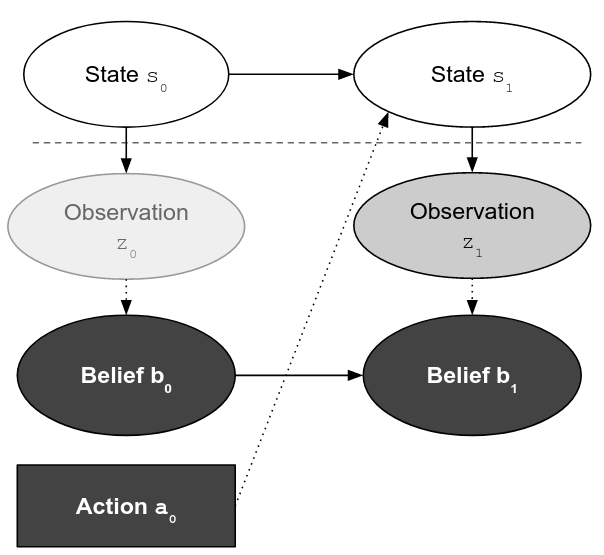
\includegraphics[width=0.5\linewidth]{figures/pomdp-state.png}
    \caption{A general process of a POMDP. True states are not available, instead, observations are received. These allow to update the agent's belief of the state that is used to choose an action to change the state towards a desired goal.}
    \label{fig:pomdp}
\end{figure}

A partially observable Markov decision process (POMDP) extends a Markov decision process (MDP) such that the agent does not directly observe the state of the environment and instead receives (partial) observations of the state.

Similar to an MDP, the state space $S$ describes the state of the environment, the action space $A$ is the set of possible actions the agent can take, the reward function $R(s, a)=r$ describes the outcome for the agent after taking an action $a \in A$ in state $s \in S$, and the transition model $T(s'|s,a)$ gives the conditional probability of the environment transitioning from state $s$ to state $s' \in S$ after the agent has taken action $a \in A$.
$\gamma \in [0,1]$ is a discount factor that describes how important future rewards are in comparison to immediate rewards when calculating total rewards.

In a POMDP, as the states are not directly available to the agent, the set of possible observations of the environment are denoted $z \in Z$ and the conditional observation model $O(z|s',a)$ assigns a probability of receiving the observation $z$ after taking action $a$ causing a transition to $s'$.
To track the state of the environment, the agent maintains a probability distribution over the state space $S$ called the belief $b$.
$b(s)$ is the probability the agent assigns to the state $s$ matching the environment's state.
Through a series of observations, the agent can update this belief to infer the state of the environment.
The goal of the agent is to find an action sequence that maximizes the expected discounted future rewards $E\left[\sum_{t=0}^\infty \gamma^t r_t \right]$ where $t$ denotes the time step of the interaction and $r_t$ is the reward at that step. 

Figure \ref{fig:pomdp} describes the interaction in a POMDP. 
Taking an action $a_0 \in A$ causes a transition of the environment's state from $s_0$ to $s_1$ with probability $T(s_1|s_0,a_0)$. 
Then, the agent receives the observation $z_1$ with probability $O(z_1|s_1,a_0)$ and a reward $r_1=R(s_1,a_0)$.
This enables the agent to update its belief from $b_0$ to $b_1$ as described in the next section.
%With a correct model of the environment and an intelligent agent, the probability of the correct state under the belief should increase $b_1(s_1) \geq b_0(s_0)$.

\subsubsection{Belief update}

We denote the operation of updating the belief from $b$ to $b'$ as $\tau(b,a,z)$.
%It depends only on the previous belief, the current action, and the current observation because the state is assumed to be Markovian.
A generic belief update can be described with Bayesian statistics.
For discrete states, the probability of a single state can then be updated using the formula:
\begin{equation}
    b'(s') = \eta \cdot O(z|s',a) \sum_{s \in S} T(s'|s,a) \cdot b(s)
    \label{eq:belief}
\end{equation}
where $\eta$ is the normalization term $1 / \sum_{s'} b'(s')$ to assert its sum is $1$.
%as the probability distribution must sum up to $1$. 
This formula must be applied to every state $s \in S$ to obtain the updated belief $b'$.
The complexity of a full belief update is then of order $O(|S|^2)$.

\subsubsection{Application to automated teaching}

This formulation can be applied to automated teaching as follows: the student represents the environment and the knowledge of the student is modeled as the state $s \in S$ that is hidden from the teaching program.
The automated teacher is the agent operating in this environment by choosing actions $a \in A$ to teach the topic.
The student responds to actions with answers $z \in Z$ that represent the observations for the automated teacher.
The automated teacher maintains a belief $b$ as a probability distribution of the knowledge of the student.
In general, its goal is to change the state of the student such that the student has mastered the topic %, although this depends on the task and context.
according to the reward function according to the pedagogical objective(s).
The original formulation by Rafferty \textit{et al.} simplifies the reward function to only depend on the action $R(a)$.

If the student's learning behavior is known, the teacher can plan and choose actions in such a way that the learning of the student is optimized. 
Such a model would thus define the transition and observation functions needed to apply the POMDP framework.


Rafferty \textit{et al.} consider that an action $a$ is the choice of a specific type of \textit{teaching activity} $t \in T$ (type) \textit{and} a specific \textit{teaching item} $i \in I$ that describes some content or example of the topic.
This decomposition allows simplifying the formulation when different teaching methods are available.
See section \ref{sec:concept-learning} for more details.


\subsubsection{Planning optimal actions}
\label{sec:planning}

Finding a policy that optimizes the pedagogical objective(s) is done via online planning, i.e., during execution. Offline planning, i.e., precomputing best actions for every possible belief state, might become computationally expensive and, thus, not tractable for longer trials or teaching tasks with a large state space. 
Hence, Rafferty \textit{et al.} employ a forward tree search algorithm with a finite horizon similar to Ross \textit{et al.}~\cite{rossPomdp2008}.

In a nutshell, the process is as follows:
The forward search starts from the current belief state $b$. 
A set of actions $\Tilde{A} \subset A$ is sampled to lower the computational cost.
Their values $q$ are calculated by simulating an interaction until horizon $d$ (depth) and the action $a^* \in A$ with the highest value is selected by the automated teacher.
%Note that we follow the convention from reinforcement learning literature to denote state values with $V$ and state-action values with $Q$.

Thus, we compute the best action $a^*_d(b)$ for a fixed horizon as follows:
\begin{equation}
    a^*_d(b) = \arg \max_{a \in \Tilde{A}} Q_d(b, a)
    \label{eq:best-action}
\end{equation}
with $b$ the current belief state, $d \in \mathbb{Z}$ the search depth, $\Tilde{A} \subset A$ the sampled actions, and $Q_d(b, a)$ the action-value function for action $a$ under the belief $b$ calculated until $d$. This follows the common notation in reinforcement learning where action-value functions are used to denote the expected reward when performing a particular action in a given state.


Since actions are composed of items $i \in I$ and teaching activity types $t \in T$, the action sampling is decomposed as follows:
$n$ teaching items $\Tilde{I} \subset I$ are sampled and the cartesian product with all teaching activity types $T$ is constructed to create $\Tilde{A} = \Tilde{I} \times T$.
The number of sampled actions is then equal to the product of sampled items and number of teaching types $|\Tilde{A}| = n \cdot |T|$.
This prevents ending up with actions of only a few types, which is very probable in the case of $|I| \gg |T|$.

A single action $a$ might cause different state changes according to $T(s'|s,a)$, and thus, different observations $z$.
For each action-observation pair, a new belief $b'=\tau(b,a,z)$ is computed.
With this new belief, the process starts anew: new actions are sampled and evaluated.
The forward search expands tree-like and grows exponentially in breadth.
To keep the computations tractable, the search is limited by a fixed depth and a reduced sample size.

% Lukas: In some way, it could be formulated to a more generic case where the empty response is part of the set of valid responses and in all cases the set is iterated but the probability of the responses result in the same result (as 0 prob for invalid responses).
If the set of possible observations following an action depends on the type of teaching activity associated with that action, we can simplify the calculation to only consider those observations that are possible for that teaching activity $Z_{i_a} \subset Z$.

To calculate the value of an action under the current belief, the future expected values of all possible observations for that action need to be considered and added to the value of the action itself. 
We compute $Q_d(b, a)$, the expected value for using the action $a \in A$ in the belief $b$ with search depth $d$ as:

\begin{equation}
    Q_d(b, a) = \begin{cases}
        R(a) + \sum_{z \in Z_{i_a}} Pr(z|b,a) \cdot \gamma \cdot V_{d-1}(b' = \tau(b, a, z)) & \, \text{if $d > 0$} \\
        \Hat{V}(b) & \, \text{if $d = 0$}
    \end{cases}
\end{equation}
with
$R(a)$ the reward for action $a$,
$Pr(z|b,a)$ the probability of receiving $z$ for action $a$ under the belief $b$,
$\gamma \in [0, 1]$ the discount factor, 
$V_d(b')$ the value function for the new belief,
and
$\Hat{V}(b)$ an estimation function of the value of the belief $b$ when the search depth is reached. 

The value of the belief $V_d(b)$ is defined as the maximum of the action-values $Q_d(b,a)$ for search depth $d$ over the sampled actions $\Tilde{A}$:
\begin{equation}
    V_d(b) = \max_{a \in \Tilde{A}} Q_d(b, a)
\end{equation}

Further, the probability of receiving an observation for an action under a belief $Pr(z|b,a)$ is simply the sum of the observation model $O(z|s,a)$ for every state, weighted by the belief probability of that state $b(s)$.
\begin{equation}
    Pr(z|b,a) = \sum_{s \in S} b(s) \cdot O(z|s,a)
\end{equation}


Finally, when the depth $d$ is reached, the value of the belief state at the leaf node is estimated by $\Hat{V}(b)$.
The specific estimation function thus needs to be defined by the task implementation of the method (see section \ref{sec:concept-learning}).
The estimated leaf value is propagated back up and discounted according to $\gamma$. 

The value of an action under a belief at a certain depth $Q_d(b,a)$ is thus the sum of the immediate reward of the action $R(a)$ and the sum over all valid observations for that action $Z_{i_a}$ of the discounted back-propagated belief state values $\gamma \cdot V_{d-1}(b')$, weighted by the observation probability $Pr(z|b,a)$.
According to the values of a set of actions, the best action $a^*_d(b)$ can be chosen according to \autoref{eq:best-action}.

%%% Lukas: Is the algorithm understandable?
\begin{algorithm}[ht]
\SetAlgoLined
\DontPrintSemicolon
\SetKwData{Input}{Data}
\KwIn{\\
\begin{tabularx}{\textwidth}{p{0.45cm}l}
    $b$      & current belief\\
    $n$      & no. of samples per level\\
    $d$      & horizon
\end{tabularx}
}
\KwOut{\\
\begin{tabularx}{\textwidth}{p{0.45cm}l}
    $v^*$     & best value of next action \\
    $a^*$     & best action
\end{tabularx}
}
\SetKwFunction{forwardsearch}{ForwardSearch}
\SetKwProg{Fn}{Function}{:}{}
\Fn{\forwardsearch{$b, n, d$}}{

$\Tilde{I} \leftarrow$ sample $n$ items uniformly from $I$\;
$\Tilde{A} \leftarrow$ $\Tilde{I} \times T$\;

$v^* \leftarrow \infty$\;

\For{$a \in \Tilde{A}$}{
    $q \leftarrow R(a)$\;
    
    \For{$z \in Z_{i_a}$}{
        $b' \leftarrow \tau(b, a, z)$\;
        
        % Lukas: It makes it easier to write the condition at this point
        % instead of in the beginning with d = 0. But this now differs from the equation formulation. Is that still okay?
        \eIf{$d = 1$}{
            $v \leftarrow \Hat{V}(b')$\;
        }{
            %%% Lukas: not sure how to represent that we only take the value
            $v \leftarrow v^*$ of \forwardsearch{$b', n, d-1$}\;
        }
        
        
        $q \leftarrow q + Pr(z|b, a) \cdot \gamma \cdot v$\;
    }
    
    \If{$q > v^*$}{
      $v^* \leftarrow q$\;
      
      $a^* \leftarrow a$\;
    }
}

\KwRet{$v^*$, $a^*$}
}
 
 \caption{Recursive forward search planning algorithm}
 \label{plan-algo}
\end{algorithm}



This algorithm is described in \autoref{plan-algo}.
It is implemented as a recursive algorithm that returns the maximum expected reward of the next action and the best action according to this reward.
In intermediate calls, the best value is used to calculate the value of the immediate action while at the top level the best action is used to define the next action to take.
For simplicity, we describe it with a single best action although in practice it is useful to maintain a list of actions with the highest known reward and choose the next action from that list. This is to prevent biasing the method toward some internal structure of the actions.

\subsection{Application as ``faster teaching'' to concept learning}
\label{sec:concept-learning}

The authors apply this general formulation to concept learning tasks.
Category or concept learning is the process of learning categories from examples~\cite{feldman2003simplicity}.

In such tasks, we denote the set of concepts as hypotheses $H$.% to better distinguish them from costs. 
The task description has to be complemented with (i) a prior distribution $p_0$ over these concepts, (ii) the items that can be used to teach the task $i \in I$, (iii) the teaching activities $t \in T$, and (iv) the possible responses $Z$.

The reward function is defined such that the teacher focuses on reducing the time needed for learning the task, hence the name ``faster teaching''. 
Each teaching action is associated with a cost (negative reward) that is modeled after the time it takes the student to complete the action. 
Thus, minimizing the costs results in the quickest learning. 
We use the cost of an action $C(a)$ and a minimization objective instead of maximizing rewards (if $R(a) = -C(a)$, then $\arg \max_a R(a) = \arg \min_a -R(a)$).

Teaching is terminated once the student has learned the concept. This is assumed if in an assessment phase the learner answers all questions correctly.
Such an assessment is performed at regular intervals to check for termination, but not used for updating the beliefs of the teacher.

\subsubsection{Teaching activity types}

In the context of concept learning, Rafferty \textit{et al.} define three possible types of teaching activity $T$: (1) showing an \textit{example}, (2) asking a \textit{quiz}, and (3) asking a question and subsequently giving \textit{feedback} about the student's response. 

\paragraph{(1) Example} In an example, the teacher presents an item with the correct result or concept. No response by the student is expected. Thus, $Z_{\text{example}} = \{\emptyset\}$. The observation model is trivial: $O(z|s,a)=1$ if $z=\emptyset$ and $0$ otherwise. However, as the example can provide new insight for the learner, the transition model assumes a state change for such cases. This change depends on the learner model and is described in the next section.

\paragraph{(2) Quiz} In a quiz, the teacher presents an item and the student has to respond with an answer.
%(in the arithmetic letter task with the correct result, and in the game number with the correct concept)
This allows the teacher to refine their belief about the student's true state, but it does not give new information to the student. 

The set of observations for this activity type contains the full set of observations valid for the concept task, $Z_{\text{quiz}} = Z$.
The definition of the observation model $O(z|s,a)$ depends on the learner model and is described in the next section. 
The transition model $T(s'|s,a)$ is trivial: as no new information is presented, the student is not expected to change their state. The transition probability is set to $1$ if both states are the same, $0$ otherwise.

\begin{equation}
    T(s'|s,a) = \begin{cases}
        1 & \, s  = s' \\
        0 & \, s \neq s'
    \end{cases}
\end{equation}

As a result, $\sum_s{T(s'|s,a) b(s)}$ of the belief update in \autoref{eq:belief} collapses to just $b(s')$.

\paragraph{(3) Feedback} In a question with feedback type of teaching activity, the previous types are combined. First, the learner is asked a question to which they respond according to their knowledge. Then, the teacher reveals whether the response was correct, and gives the correct answer in case of an incorrect answer. 
Here, both the observation model and the transition model are used in a non-trivial way. 
As in the \textit{quiz}, the set of observations for this teaching activity contains the full set of observations valid for the concept task, $Z_{\text{feedback}} = Z$, and the observation model $O(z|s,a)$ depends on the learner model. 
And as in the \textit{example}, the transition model depends on the learner model, as the feedback can provide new information to the learner.

Note that when modeling the update as in the Bayesian belief formula (\ref{eq:belief}), the update has to be split into two separate steps: the response of the learner is always related to the state before taking the action, while the feedback might trigger a state change without an additional observation. So first, the belief update according to the response $z$ has to be calculated in the same way as in the \textit{quiz} activity. Second, if the response was incorrect, a state change is expected based on the true answer, as in the \textit{example} activity type.

\vspace{3mm}
To reflect these similarities between the feedback type and the other activity types, we will use \textit{refinement activities} to refer to the quiz activity and the question part of the feedback activity (as they both allow the teacher to refine the belief), and \textit{evidence activities} to refer to the example activity and the feedback part of the feedback activity (as they both allow the learner to improve its knowledge). 

We define the generic belief update formulas for \textit{refinement} and \textit{evidence activities} as:

\begin{equation}
    b'(s') = \begin{cases}
        \eta \cdot O(z|s',a) \cdot b(s')    & \, \text{for refinement activities} \\
        \eta \cdot \sum_{s \in S} T(s'|s, a) \cdot b(s)    & \, \text{for evidence activities}
    \end{cases}
    \label{eq:belief-update-types}
\end{equation}

$\eta$ refers to the normalization term and depends on the belief formula.

Finally, we denote by $H_a$ the set of concepts (hypotheses) that are consistent with action $a$, and $H_{z \mid a}$ the set of concepts which imply that $z$ is a correct answer to action $a$. 

\subsection{Learner models}

The learner model defines the details of the transition and observation functions.
Rafferty \textit{et al.} postulate three learner models: (1) a discrete memoryless model, (2) a discrete model with memory, and (3) a continuous model with a dynamic probability distribution over the concept space. All models are extended to include noise to accommodate human error during the learning.


\paragraph{Noise} Two types of noises are added to all models: a production noise $\epsilon_p$ for cases where the student responds inconsistently to their knowledge, and a transition noise $\epsilon_t$ for cases where the student ignores new evidence and does not transition to a new consistent state.
For the production noise, it is assumed that the student responds with a random answer drawn uniformly from all possible answers. 
The transition noise affects the state transitions, and the models need to incorporate this behavior in their updating rules to prevent diverging beliefs and states.

\paragraph{(1) Memoryless model}
This model is close to the learning model of Restle \textit{et al.} \cite{restle1962selection} and assumes that no explicit memory of previous actions is kept while storing a specific concept hypothesis that is currently believed to be true by the learner (as opposed to considering multiple possible plausible concepts).
Thus, the learner state only depends on the current knowledge and the immediate teaching activity.
The state space $S$ is isomorphic to the space of possible concepts $H$, such that any $s\in S$ corresponds to one specific concept hypothesis denoted $h_s$.

For refinement activities, the observation model needs to be defined.
As the learner holds a single true concept, the response corresponds to the result under this single concept.
Taking noise into account, the observation model is defined as follows:
\begin{equation}
    O(z|s,a) = \begin{cases}
        (1-\epsilon_p)+\frac{\epsilon_p}{|Z_{i_a}|}    & \, \text{if $z$ is consistent for $a$ under $s$} \\
        \frac{\epsilon_p}{|Z_{i_a}|}                   & \, \text{otherwise}
    \end{cases}
\end{equation}
with $\frac{\epsilon_p}{|Z_{i_a}|}$ the probability of choosing a random response in case of a production error.


For evidence activities, the learner is assumed to transition to a concept consistent with the new evidence if not already in a consistent state. The probability of each consistent concept is proportional its prior probability. 
% Lukas: removed as not necessary really, right? We can go directly to the noisy definition
% \begin{equation}
%     T(s'|s,a) \propto
%     \begin{cases}
%         p_0(h_{s'}) & \, \text{if $h_{s'} \in H_{a}$} \\
%         0       & \, \text{otherwise}
%     \end{cases}
% \end{equation}
% with $p_0$ the prior probability over the possible concepts.
With noise, the transition model is defined as follows:
\begin{equation}
    T(s'|s, a) = \begin{cases}
        1       & \, \text{if } h_{s'} \in H_a \text{ and } s' = s, \\ %s'=s consistent, already in the same consistent state
        (1 - \epsilon_t) \cdot \dfrac{p_0(h_{s'})}{\sum_{s'' \mid h_{s''} \in H_a} p_0(h_{s''})} & \, \text{if } h_{s'} \in H_a \text{ and } s' \neq s, \\ %s' consistent, s inconsistent
        \epsilon_t & \, \text{if }  h_{s'} \notin H_a \text{ and } s' = s, \\ %s'=s inconsistent
        0 & \, \text{otherwise}
    \end{cases}
    \label{eq:trans-model}
\end{equation}
with $p_0$ the prior probability over the possible concepts,
and $\frac{p_0(h_{s'})}{\sum_{s'' \mid h_{s''} \in H_a} p_0(h_{s''})}$ the probability of going from an inconsistent state to a particular consistent state based on the relative prior among the consistent states.

%This implies that the learner stays with probability $\epsilon_t$ in states inconsistent with the new evidence provided by the action.

The sum over states in \autoref{eq:belief-update-types} for evidence actions can be decomposed to accommodate this structure.
For states consistent with the information provided by the action, it is composed of two parts: the likelihood of transitioning from an inconsistent state to this consistent state, and the likelihood of already being in this state and, thus, not transitioning.
The belief update is consequently:
\begin{equation}
    b(s')= \begin{cases}
        \eta \cdot \left[(1 - \epsilon_t) \cdot \frac{p_0(h_{s'})}{\sum_{s \mid h_s \in H_a}{p_0(h_s)}} \cdot \sum_{s \mid h_s \notin H_a}{b(s)}\right] + b(s') & \text{if } h_{s'} \in H_a \\
        \eta \cdot \epsilon_t \cdot b(s') & \text{ otherwise }
    \end{cases}
\end{equation}

Note, that in case of feedback activities, the evidence update only has to be performed for incorrect answers, as the learner is assumed to not transition for correct responses.


\paragraph{(2) Discrete model with memory}
%%% Lukas: Actually, there is no reference for this model cited in the original paper
This model extends the memoryless model so that a history of the past $m$ actions is kept.
Transitions then have to be consistent with the current action plus the memory actions, denoted $A_M$.
The memory only needs to store actions that contain information, i.e., quiz activities are ignored.
As for the memoryless model, it is assumed that the student only holds a single concept as true and responds accordingly to it.


If the memory would not be perfect, it must be considered part of the student's state.
In this case, the number of possible memory states $S_M$ is calculated based on the set of teaching items $I$ and the set of valid memory teaching activities $T_{mem}$ as $|S_M| = \sum_{k=0}^m |I \times T_{mem}|^k$.
%While $|I \times T_{mem}|^m$ represents the memory states where all slots are filled, the lower powers represent those states where some slots are not filled which can only occur on one side.
Taken together, the total state space would increase by the memory states and become $|S|=|H| \cdot |S_M|$ resulting in a possibly huge state space.
For example, in the letter arithmetic task with 6 letter-number pairs, 15 teaching items, 2 valid memory teaching activities, and a memory size of $2$, the total number of memory states would grow from $|H|=720$ to $|H|\cdot (1 + 30 + 30^2) =670.302$.


However, the model assumes a `flawless' memory, i.e., even if an action is ignored for updating the state due to the transition noise, it is kept in memory. As a consequence, at every time step, only the single memory state based on the action history is possible and needs to be considered, reducing the state space to $|H|$ as before.

The transition and observation models are formulated analogously to the memoryless case. 
The only difference is that the set of consistent concepts with the current action $H_a$ has to be consistent also with the actions in memory $A_M$.

\paragraph{(3) Continuous model}
This model assumes that the student maintains a probability distribution over all possible solutions as formulated in \cite{tenenbaum2000rules}. 
No explicit history of previous actions is stored but the state contains implicit information about the history.
In this case, every state is a probability distribution over all elements of $H$, making the state space infinitely large. Thus, approximations are needed to make this model feasible.

In this model, a state consistent with an action-observation pair is one in which the probabilities of all inconsistent concepts with the action is zero $p_s(h \notin H_a) = 0$.

Responses to teaching actions are probabilistic and correspond to the combined probability the student places on the concepts with $z$ as a correct answer.

\begin{equation}
    O(z|s,a) = \sum_{h \in H_{z \mid a}} p_s(h)
\end{equation}

where $p_s(h)$ is the probability of the hypothesis $h$ in the state $s$.

The transition model is defined such that for new evidence, the learner transitions deterministically to the closest consistent derivation of the current state $s$.
This derived state $s_a^*$ for the current action $a$ is a copy of the current state in which the probabilities of all inconsistent hypotheses are set to $0$ while the other probabilities are retained and normalized.

\begin{equation}
    T(s'|s,a) = \begin{cases}
        1     & \, \text{if $s$ is consistent with $a$ and $s' = s$} \\
        1     & \, \text{if $s$ is inconsistent with $a$ and $s' = s_a^*$} \\
        0     & \, \mathrm{otherwise}
    \end{cases}
    \label{eq:cont-ps}
\end{equation}

With diverse evidence, the probability distribution converges to the true concept.

From the perspective of the teacher, it is intractable to hold a belief over the infinite set of states. Below, we review the particle filter implementation that is employed instead.

\paragraph{\textit{Particle filter}}
A particle filter is used to approximate the infinite set of possible states via a limited number of weighted particles \cite{DoucetSeqMCM2001}.
In this particle filter, each particle $p \in P$ represents one possible state $s_p$ (i.e., a probability distribution over concepts), and the weight $w_p$ indicates the probability the teacher assigns to this particle.
The sum of the weights must always be $1$ as in a probability distribution.
The particles $P$ can be thought of as corresponding to $b$ and the weights to $b(s)$ in the discrete case.
As the belief state is approximated, the belief update $\tau(b,a,z)$ is now a function of the existing particles as described below.

In the beginning, the particles are initialized with two particles sharing equal weight: one particle corresponding to the prior distribution $p_0$, and one particle with a uniform distribution over the concepts. 
If the prior distribution is uniform, only one particle is created.

After each action, the particles are updated, and new particles are created based on the observation and transition models, and their weights are recalculated.
This corresponds to the belief updates in the discrete models.

For \textit{refinement activities}, the weights of the particles are updated based on the observation model as follows:

\begin{equation}
    w_p' = \eta \cdot w_p \cdot O(z|s,a)
\end{equation}

\begin{equation}
    O(z|s,a) = (1 - \epsilon_p) \cdot \sum_{h \in H_{z\mid a}}{p_{s_p}(h)} + \frac{\epsilon_p}{|Z_{i_a}|}
\end{equation}
with $\frac{\epsilon_p}{|Z_{i_a}|}$ being the probability of observing the response $z$ due to a production error.
$\eta$ now refers to the renormalization factor after processing all particles, $1 / \sum_{p \in P}{w_p}$.
This corresponds to the regular belief update \autoref{eq:belief-update-types}.

For actions using an \textit{evidence activity}, every particle is replaced by two new particles, one assuming the learner did not transition, and one assuming the learner transitioned.
The non-transitioned particle is simply a copy of the previous particle, with the weight adjusted by $\epsilon_t$.
The transitioned particle is based on the old particle and updated to reflect the new evidence. For this, the probability for all inconsistent states is set to zero $p_{s_p}(h \notin H_a) \leftarrow 0$.
The weight of both particles is thus updated according to:

\begin{equation}
    w_p' = \begin{cases} 
        \eta \cdot (1 - \epsilon_t) \cdot w_p & \, \text{for transitioned particles} \\
        \eta \cdot \epsilon_t \cdot w_p & \, \text{for non-transitioned particles}
    \end{cases}
\end{equation}

Since this update doubles the number of particles, there is a limit imposed to prevent uncontrolled growth on the number of particles.
If the total number of particles exceeds some predefined maximum, the particles with the smallest weight are removed so that the limit is satisfied, and the weights are normalized again.


The weight updates and renormalizations are performed after both \textit{refinement} and \textit{evidence} activities separately (relevant in the case of \textit{feedback} activities).
Further, in both cases, there is a check for \textit{particle depletion} (i.e., no particle is probable).
This happens if the sum\footnote{Note that it is always the \textit{sum} and not the maximum of the weights as wrongly stated in one passage in the original supplementary material (as confirmed from the original implementation).} of all particle weights is below some threshold.
In this case, all particles are eliminated, and two new particles are initialized with equal weight.
One particle is created according to the prior distribution and the other particle according to the state a learner without noise would have ended up in following the history of previously seen actions. 

In this model, the update based on new evidence has to be done also for correct responses to feedback activities, as the response is sampled from the state of the learner and does not represent a certain answer.

\subsubsection{Planning}

For every learner model, a corresponding policy is constructed that follows the forward tree search planning algorithm described in section \ref{sec:planning}.
To estimate the cost of the leaf nodes in such concept learning tasks, 
the authors take the probability of failing the assessment phase (given by the belief) and multiply it by a scaling of the minimum future costs:

\begin{equation}
    \Hat{V}(b) = (1 - p_b(h_{true})) \cdot \alpha \cdot \min_a{C(a)}
    \label{eq:leaf-calc}
\end{equation}
with $p_b(h_{true})$, the probability assigned to the true concept in the current belief, and $\alpha$ a scale parameter. 

For the memoryless and the model with memory, $p_b(h_{true})$ is simply the belief probability of the true concept. 
For the continuous model, it is the combined probability of the true concept of all particles, weighted by the corresponding particle weight.

\begin{equation}
    p_b(h_{true} \mid b) = \begin{cases}
        b(s = h_{true}) & \, \text{for the discrete models} \\
        \sum_{s_p \mid p \in P}{w_{s_p} \cdot p_{s_p}(h_{true})} & \, \text{for the continuous model}
    \end{cases}
\end{equation}

\subsection{Comparison with original paper}

We tried to honor the original method description as much as we could.
While certain elements were not clear to us, we discussed open questions with the first author of the original paper, and verified certain assumptions with their implementation.
Specifically, we verified that one should compute the belief update without the explicit Bayesian equation (\ref{eq:belief}), and treat the belief update as a two-step process for the refinement and evidence parts of the actions, which is especially relevant for the \textit{feedback} activity.
% This led us to handle it as a combination of the other two activities.
We deduced the planning algorithm \ref{plan-algo} from the referenced papers and validated it with the original implementation, and verified that the memory is not part of the state in the discrete model with memory, and that the memory ignores quizzes.
% Finally, as well as the handling of noises in the learner models, and how they are treated in the respective equations.
As such, we did not have to take design decisions as clarifications were provided by the original authors.
Still, there might be differences in implementation details as we focused our validation on the conceptual algorithms and model equations.
